\documentclass{article}

\usepackage{xstring}
\usepackage{fancyhdr}
\usepackage{extramarks}
\usepackage{amsmath}
\usepackage{amsthm}
\usepackage{amsfonts}
\usepackage{tikz}
\usepackage[plain]{algorithm}
\usepackage{algpseudocode}
\usepackage{parskip}
\usepackage{enumerate}
\usepackage{setspace}
\usepackage{subfig}
\usepackage{listings}
\usepackage{pgfplots}
\usepackage{url}
\usetikzlibrary{arrows,shapes,positioning,shadows,trees}

%
% Basic Document Settings
%

\topmargin=-0.45in
\evensidemargin=0in
\oddsidemargin=0in
\textwidth=6.5in
\textheight=9.0in
\headsep=0.25in

\linespread{1.1}

\pagestyle{fancy}
\lhead{\hmwkAuthorName}
\chead{\hmwkClass\ (\hmwkClassInstructor): \hmwkTitle}
\rhead{\firstxmark}
\lfoot{\lastxmark}
\cfoot{\thepage}

\renewcommand\headrulewidth{0.4pt}
\renewcommand\footrulewidth{0.4pt}

\setlength\parindent{0pt}

\tikzset{
    raw sort entry/.style={rectangle, thick, draw, node distance=1.5em, align=center},
    sort entry black/.style={raw sort entry, black, fill=white, align=center},
    p1/.style={raw sort entry, black, fill=gray!25},
    s1/.style={raw sort entry, red, fill=yellow!30},
    s2/.style={raw sort entry, blue, fill=green!20},
    s3/.style={raw sort entry, violet, fill=orange!25},
    basic/.style  = {draw, font=\sffamily, rectangle},
    root/.style   = {basic, rounded corners=2pt, thin, align=center},
    level 2/.style = {basic, rounded corners=6pt, thin,align=center},
    level 3/.style = {basic, thin, align=left}
}

\newcommand*{\List}[2][sort entry black]{%
  \par\noindent%
  \edef\listtoprocess{#2}%
  \def\ListToProcess{}%
  \begin{center}
  \begin{tikzpicture}[inner sep=2pt, outer sep=0]
    \foreach \content in \listtoprocess{
      \IfSubStr{\content}{/}{% true
        \xdef\ListToProcess{\ListToProcess,\content}
      }{%                      false
        \xdef\ListToProcess{\ListToProcess,#1/\content}
      }
    }
    \StrGobbleLeft{\ListToProcess}{1}[\ListToProcess]% removes the first comma (\listToProcess is empty at the start)
    \foreach [count=\i] \Style/\Value in \ListToProcess {
      \ifnum\i=1\relax
        \node [raw sort entry, \Style] (sortnode\i) {\Value};
      \else
        \node [raw sort entry, right of=sortnode\number\numexpr\i-1\relax, \Style] (sortnode\i) {\Value};
      \fi
    }
  \end{tikzpicture}%
  \end{center}
}

%
% Create Problem Sections
%

\newcommand{\enterProblemHeader}[1]{
    \nobreak\extramarks{}{Problem \arabic{#1} continued on next page\ldots}\nobreak{}
    \nobreak\extramarks{Problem \arabic{#1} (continued)}{Problem \arabic{#1} continued on next page\ldots}\nobreak{}
}

\newcommand{\exitProblemHeader}[1]{
    \nobreak\extramarks{Problem \arabic{#1} (continued)}{Problem \arabic{#1} continued on next page\ldots}\nobreak{}
    \stepcounter{#1}
    \nobreak\extramarks{Problem \arabic{#1}}{}\nobreak{}
}

\setcounter{secnumdepth}{0}
\newcounter{partCounter}
\newcounter{homeworkProblemCounter}
\setcounter{homeworkProblemCounter}{1}
\nobreak\extramarks{Problem \arabic{homeworkProblemCounter}}{}\nobreak{}

%
% Homework Problem Environment
%
% This environment takes an optional argument. When given, it will adjust the
% problem counter. This is useful for when the problems given for your
% assignment aren't sequential. See the last 3 problems of this template for an
% example.
%
\newenvironment{homeworkProblem}[1][-1]{
    \ifnum#1>0
        \setcounter{homeworkProblemCounter}{#1}
    \fi
    \section{Problem \arabic{homeworkProblemCounter}}
    \setcounter{partCounter}{1}
    \enterProblemHeader{homeworkProblemCounter}
}{
    \exitProblemHeader{homeworkProblemCounter}
}

%
% Homework Details
%   - Title
%   - Due date
%   - Class
%   - Section/Time
%   - Instructor
%   - Author
%

\newcommand{\hmwkTitle}{Sorting Algorithms}
\newcommand{\hmwkDueDate}{February 26, 2015}
\newcommand{\hmwkClass}{CS350 - Algorithms}
\newcommand{\hmwkClassInstructor}{for Professor Andrew Black}
\newcommand{\hmwkAuthorName}{Kristina Frye}

%
% Title Page
%

\title{
    \vspace{2in}
    \textmd{\textbf{\hmwkClass:\ \hmwkTitle}}\\
    \normalsize\vspace{0.1in}\small{Due\ on\ \hmwkDueDate}\\
    \vspace{0.1in}\large{\textit{\hmwkClassInstructor}}
    \vspace{3in}
}

\author{\textbf{\hmwkAuthorName}}
\date{}

\renewcommand{\part}[1]{\textbf{\large Part \Alph{partCounter}}\stepcounter{partCounter}\\}

%
% Various Helper Commands
%

% Useful for algorithms
\newcommand{\alg}[1]{\textsc{\bfseries \footnotesize #1}}

% For derivatives
\newcommand{\deriv}[1]{\frac{\mathrm{d}}{\mathrm{d}x} (#1)}

% For partial derivatives
\newcommand{\pderiv}[2]{\frac{\partial}{\partial #1} (#2)}

% Integral dx
\newcommand{\dx}{\mathrm{d}x}

% Alias for the Solution section header
\newcommand{\solution}{\textbf{\large Solution}}

% Probability commands: Expectation, Variance, Covariance, Bias
\newcommand{\E}{\mathrm{E}}
\newcommand{\Var}{\mathrm{Var}}
\newcommand{\Cov}{\mathrm{Cov}}
\newcommand{\Bias}{\mathrm{Bias}}

\begin{document}

\pagebreak



\section{Mergesort}
Mergesort is a divide-and-conquer algorithm in which the unsorted array is recursively divided
in half until each subarray has only one element. After this phase is completed, the pieces are 
merged back together in order, eventually recombining into one sorted array. See 
Figure~\ref{pseudo-mergesort} for the pseudocode representation of Mergesort.

In the first phase of Mergesort, the elements of the array are copied $\log_2(n)$ times until each 
element is in its own subarray. Although no comparisons are made in this phase of the algorithm,
this does require $n\log_2 n$ copy operations (each element is copied $\log_2n$ times) 
and doubles the required space allocation for the array.

In the second phase of Mergesort, the elements of each subarray are combined: the first elements of each subarray are compared and the smaller element is moved from its subarray into the sorted array. In the worse case, the subarrays are alternately reduced by one, leading to a total of $n-1$
comparisons. Adding these comparisons to the comparisons required to create each subarray 
results in the following recurrence:
\[
	C(n) = 2 \cdot C\left(\frac{n}{2}\right) + n-1, C(1) = 0
\]
This recurrence is conveniently in the form of the Master Theorem in which
\[
	T(n) = a \cdot T\left(\frac{n}{b}\right) +f(n)
\]
and $f(n) \in \Theta(n^d)$. For Mergesort, $a = 2, b = 2, d = 1$ and $a = 2 = 2^1 = b^d$. 
Therefore, according to the Master Theorem, $C(n) \in \Theta(n^d \log n)$. However, in many
cases, there will less than $n-1$ comparisons in each merge. For instance, if
all the elements of the left subarray are less than all the elements of the right array, the left
subarray will be repeatedly reduced after each comparison. After $\frac{n}{2}$ comparisons 
have been performed, the left subarray will be empty, and all the elements of the right subarray 
can simply be copied to the sorted array without any further comparisons. 
See line~\ref{line:mergesort1} through line~\ref{line:mergesort2} in Figure~\ref{pseudo-mergesort}.
Figure~\ref{example-mergesort} shows an example of an array of numbers being sorted with Mergesort.

Mergesort has many advantages. First, of all the ``good'' sorting algorithms, Mergesort is probably
the easiest to understand and thus implement. Second, its worst case is better than the worst
case of Quicksort, which is generally considered a faster algorithm. But its main advantage is that,
unlike many other sorting algorithms, it is a \textit{stable} sort. That is, two elements that are equal 
to each other will remain in the same relative order after the algorithm has been completed. This
can be important when performing repeated searches of different aspects of the same objects.
For instance, when sorting names, it is common to sort by first name and then by last name.
If the sort is stable, the first names will remain in order while the last names are sorted, resulting
in names in a correct final sort. An unstable sorting algorithm would be unsuitable for this
type of sorting problem.

Mergesort has two main disadvantages. First, it requires a large number of copy operations in both
phases of the algorithm. Second, it requires $O(n)$ of extra space and cannot be performed 
in place. That said, its simplicity, relative speed, and stability make it a good sorting algorithm
for many applications.

\begin{figure}
\begin{algorithmic}[1]
	\Procedure{Mergesort}{$A[0..n-1]$}
		\State $left \gets A[0..n/2]$
		\State $right \gets A[n/2 + 1..n-1]$
		\State $left \gets Mergesort(left)$
		\State $right \gets Mergesort(right)$
		\State $A \gets merge(left, right, A)$
	\EndProcedure
	
	\Procedure{Merge}{$left, right, A$}
		\State $i \gets 0$
		\State $j \gets 0$
		\State $k \gets 0$
		\While{$i < left.length$ AND $j < right.length$}
			\If {$left[i] < right[j]}$
				\State $A[k] \gets left[i]$
				\State $i \gets i + 1$
			\Else
				\State $A[k] \gets right[j]$
				\State $j \gets j + 1$
			\EndIf
			\State $k \gets k + 1$
		\EndWhile
		\If {$i = left.length$} \label{line:mergesort1}
			\State copy $right[j..right.length - 1]$ to $A[k..left.length + right.length - 1]$
		\Else
			\State copy $left[i..left.length - 1]$ to $A[k..left.length + right.length - 1]$
		\EndIf \label{line:mergesort2}
		\State return $A$
	\EndProcedure
\end{algorithmic}
\caption{Pseudocode for Mergesort}
\label{pseudo-mergesort}
\end{figure}
	
\begin{figure}[mergesort] \begin{center}
	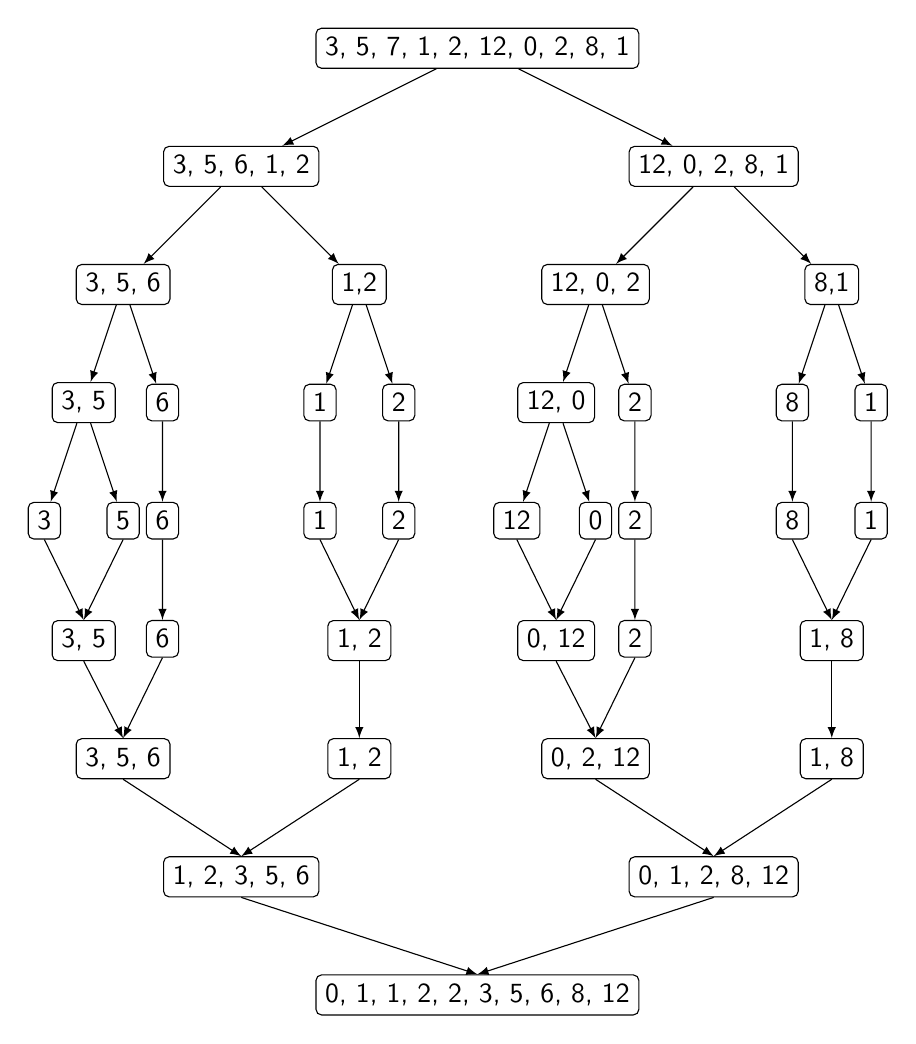
\begin{tikzpicture}[
	level 1/.style={sibling distance=60mm},
	level 2/.style={sibling distance=30mm},
	level 3/.style={sibling distance=10mm},
	edge from parent/.style={->,draw},>=latex]
		\begin{scope}[every node/.style={root}]
			\node(node35712120281){3, 5, 7, 1, 2, 12, 0, 2, 8, 1}
			child {node(node35612){3, 5, 6, 1, 2}
				child {node(node356-1){3, 5, 6}
					child{node(node35-1){3, 5}
						child{node(node3){3}}
						child{node(node5){5}}}
					child{node{6}
						child{node{6}
						child{node(node6){6}}}}}
				child {node(node12-1){1,2}
					child{ node{1}
						child{ node(node1){1}}}
					child{ node{2}
						child{ node(node2){2}}}}}
			child {node(node120281){12, 0, 2, 8, 1}
				child {node(node1202){12, 0, 2}
					child{ node(node120){12, 0}
						child{ node(node12-4){12}}
						child{ node(node0){0}}}
					child{ node{2}
						child{ node{2}
							child{ node(node2-2){2}}}}}
				child {node(node81){8,1}
					child{ node{8}
						child{ node(node8){8}}}
					child { node{1}
						child{ node(node1-2){1}}}}};
		\node[below = 2.5 of node35-1](node35-2){3, 5};
		\draw[->] (node3.south) --  (node35-2.north);
		\draw[->] (node5.south) --  (node35-2.north);
		
		\node[below = 4 of node12-1](node12-2){1, 2}
			child{ node(node12-3){1, 2}};
		
		\node[below = 2.5 of node120](node012){0, 12};
		\draw[->] (node12-4.south) --  (node012.north);
		\draw[->] (node0.south) --  (node012.north);
		\draw[->] (node1.south) --  (node12-2.north);
		\draw[->] (node2.south) --  (node12-2.north);
		
		\node[below = 4 of node81](node18){1, 8}
			child{ node(node18-2){1, 8}};
		\draw[->] (node8.south) --  (node18.north);
		\draw[->] (node1-2.south) --  (node18.north);
		
		\node[below = 5.5 of node1202](node0212){0, 2, 12};
		\draw[->] (node012.south) --  (node0212.north);
		\draw[->] (node2-2.south) --  (node0212.north);
		
		\node[below = 5.5 of node356-1](node356-2){3, 5, 6};
		\draw[->] (node35-2.south) --  (node356-2.north);
		\draw[->] (node6.south) --  (node356-2.north);
		\node[below = 8.5 of node35612](node12356){1, 2, 3, 5, 6};
		\draw[->] (node356-2.south) -- (node12356.north);
		\draw[->] (node12-3.south) -- (node12356.north);
		
		\node[below = 8.5 of node120281](node012812){0, 1, 2, 8, 12};
		\draw[->] (node0212.south) -- (node012812.north);
		\draw[->] (node18-2.south) -- (node012812.north);
		
		\node[below = 11.5 of node35712120281](end){0, 1, 1, 2, 2, 3, 5, 6, 8, 12};
		\draw[->] (node12356.south) -- (end.north);
		\draw[->] (node012812.south) -- (end.north);
		\end{scope}
	\end{tikzpicture} \caption{An example of Mergesort} \label{example-mergesort}
\end{center} \end{figure}
\pagebreak

\section{Heapsort}
A heap is a type of binary tree that is implemented within an array. It has a couple of important
properties such as being complete (although there may be empty nodes in the right leaves of the
last level) and having parental dominance. That is, each parent node has a larger value than either of the child nodes. 

The heap nodes are constructed from the array indices as shown in Figure~\ref{heap}. That is,
the first element of the array corresponds to the root node, the second and third elements go
into the immediate children of the root node, and so forth. Therefore, all the interior nodes
are located in the indices that are equal to less than $(n-1)/2$. That is, in an array with seven
elements, the indices of the array that are less than 3 (0, 1, 2) are in the interior nodes. Nodes
equal to and greater than 3 are located in the leaves of the heap.

This is important because we "heapify" an array by heapifying each interior node, starting from the
last one. That is, each node is compared against its child nodes. If a child has a larger value,
it is switched with the parent node. This process is described in pseudocode in Figure~\ref{heapify}.
Once the array has been turned into a heap, the largest value will be in the node of the heap, which
is the first element of the array. To sort the array, the first element of the array is switched with the
last element of the array, and the new first element is run through the $heapify$ procedure
again, minus the last element of the array. This process is completed until there is only one
element left to be heapified. At this point, the array is sorted. See Figure~\ref{heapsort}.

Figure~\ref{example-heapsort1} and Figure~\ref{example-heapsort2} show a step-by-step
example of the second phase of Heapsort. The list of numbers corresponds to the array
that is the process of being sorted. The tree below each list shows the corresponding
heap after the heapify process has been completed. The algorithm is complete when there is
only one element left to heapify.

To calculate the algorithmic efficiency of Heapsort, consider both phases of the algorithm.
In the first phase, the array is heapified by iterating through each internal node and recursing
through its children. Let $n$ be the number of nodes with $n = 2^{h+1} - 1$ where $h$ is the height 
of the tree. When examining a node, two comparisons are made: 
one between the node's children, and one between the maximum child and the node itself. If the 
node switches with its child, another two comparisons are made with the child and its children and so 
on for the height of the tree, resulting in $2(h-i)$ total comparisons for that node. There are $2^h$ 
nodes per level. Therefore, the number of comparisons that are made are:
\begin{align*}
	C(h) &= \sum_{i=0}^{h-1} 2(h-i) 2^i = \sum_{j=1}^{h}2j 2^{h-j} = 2 \sum_{j=1}^h \frac{j2^h}{2^j}\\
	&= 2^{h+1} \sum_{j=1}^h \frac{j}{2^j} \le 2^{h+1}\sum_{j=1}^{\infty} \frac{j}{2^j}
\end{align*}
But 
\[
	\sum_{j=1}^{\infty} \frac{j}{2^j} = 2.
\]
So:
\[
	C(h) \le 2^{h+1} \cdot 2 = 2(n + 1) \in O(n)
\] 
In the second phase, the first node is swapped with the last node, and heapify is performed on
the new first node, which involves two comparisons a level for up to the height of the tree. 
This equals $2 \log_2(n-1)$ comparisons with $n$ getting smaller with each iteration. 
\[
	\sum \log_2 n \in O(n \log n)
\]
Therefore, the total number of comparisons for Heapsort is $O(n) + O(n\log n) = O(n\log n).$

Unlike Mergesort, Heapsort does not require any additional space and can be performed
completely in place. It is an iterative algorithm as opposed to a recursive algorithm, which
can be an important characteristic for some types of inputs. This will be discussed in some 
detail later in the paper.

\begin{figure}[heap]
	\begin{center}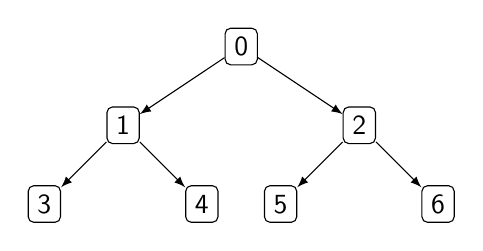
\begin{tikzpicture}[
	level 1/.style={sibling distance=30mm},
	level 2/.style={sibling distance=20mm},
	level 3/.style={sibling distance=10mm},
	level distance=1cm,
	edge from parent/.style={->,draw},>=latex]
		\begin{scope}[every node/.style={root}]
			\node{0}
				child{node{1}
					child{node{3}}
					child{node{4}}}
				child{node{2}
					child{node{5}}
					child{node{6}}};
		\end{scope}
	\end{tikzpicture}
	\caption{Constructing a heap. The numbers shown in the nodes correspond to the array indices.}
	\label{heap}\end{center}
\end{figure}

\begin{figure}
\begin{algorithmic}[1]
	\Procedure{heapify}{$A[lo..length], root, lo, length)$}
		\State $temp \gets A[lo + root - 1]$
		\While{$root * 2 \le high$}
			\State $child \gets 2 * root$
			\If{$child < length$ AND $A[lo + child - 1] \le A[lo + child]$}
				\State $child \gets child + 1$ 
				\Comment{Choose the larger child}
			\EndIf
			\If{$temp \ge A[lo + child - 1]$}
				\State break 
				\Comment{If parent is bigger than largest child then done}
			\EndIf
			\State $A[lo + root - 1] = A[lo + child - 1]$
			\State $root = child$ 
			\Comment{The child needs to be checked now}
		\EndWhile
		\State $A[lo + root - 1] \gets temp$
	\EndProcedure
\end{algorithmic}
\caption{The process of heapifying an element of an array}
\label{heapify}
\end{figure}

\begin{figure}
\begin{algorithmic}[1]
	\Procedure{Heapsort}{$A[lo..high], lo, high$}
		\State $length \gets high - lo$
		\For {$i := length/2 \text{ to } 1 \textbf{ step } {-1}$}
			\State $heapify(A, i, lo, length)$
		\EndFor
		\For {$i := length \text{ to } 1 \textbf{ step }{-1}$}
			\State $swap(A, lo, lo + i - 1)$
			\State $heapify(A, 1, lo, i-1)$
		\EndFor
	\EndProcedure
\end{algorithmic}
\caption{Heapsort}
\label{heapsort}
\end{figure}

\begin{figure}
	\List{3, 5, 7, 1, 2, 12, 0, 2, 8, 1}
	\vspace{5mm}
	\begin{center}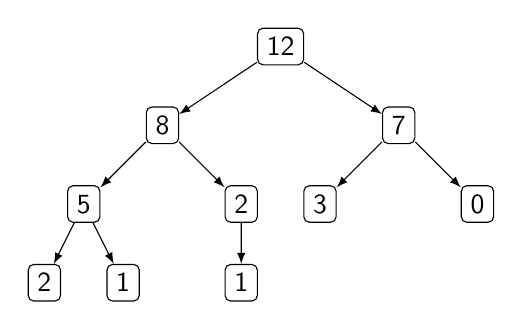
\begin{tikzpicture}[
	level 1/.style={sibling distance=30mm},
	level 2/.style={sibling distance=20mm},
	level 3/.style={sibling distance=10mm},
	level distance = 1cm,
	edge from parent/.style={->,draw},>=latex]
		\begin{scope}[every node/.style={root}]
			\node{12}
				child{node{8}
					child{ node{5}
						child{ node{2}}
						child{ node{1}}}
					child{ node{2}
						child{ node{1}}}}
				child{ node{7}
					child{ node{3}}
					child{ node{0}}};	
		\end{scope}
	\end{tikzpicture}\end{center} 
	\vspace{5mm}
	\List{1, 8, 7, 5, 2, 3, 0, 2, 1, 12}
	\vspace{5mm}
	\begin{center}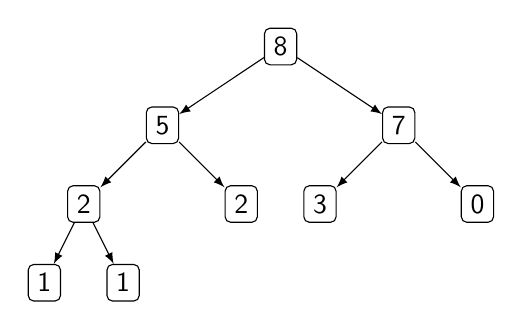
\begin{tikzpicture}[
	level 1/.style={sibling distance=30mm},
	level 2/.style={sibling distance=20mm},
	level 3/.style={sibling distance=10mm},
	level distance = 1cm,
	edge from parent/.style={->,draw},>=latex]
		\begin{scope}[every node/.style={root}]
			\node{8}
				child{node{5}
					child{node{2}
						child{node{1}}
						child{node{1}}}
					child{node{2}}}
				child{node{7}
					child{node{3}}
					child{node{0}}};
		\end{scope}
	\end{tikzpicture}\end{center} 
	\vspace{5mm}
	\List{1, 5, 7, 2, 2, 3, 0, 1, 8, 12}
	\vspace{5mm}
	\begin{center}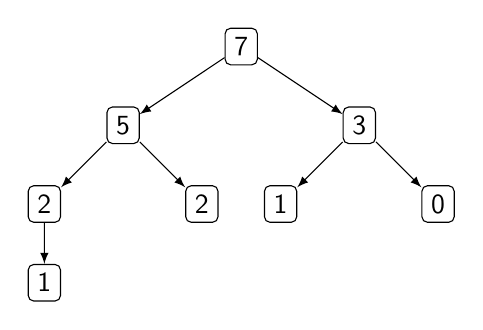
\begin{tikzpicture}[
	level 1/.style={sibling distance=30mm},
	level 2/.style={sibling distance=20mm},
	level 3/.style={sibling distance=10mm},
	level distance = 1cm,
	edge from parent/.style={->,draw},>=latex]
		\begin{scope}[every node/.style={root}]
			\node{7}
				child{node{5}
					child{node{2}
						child{node{1}}}
					child{node{2}}}
				child{node{3}
					child{node{1}}
					child{node{0}}};
		\end{scope}
	\end{tikzpicture}\end{center} 
	\vspace{5mm}
	\List{1, 5, 3, 2, 2, 1, 0, 7, 8, 12}
	\vspace{5mm}
	\begin{center}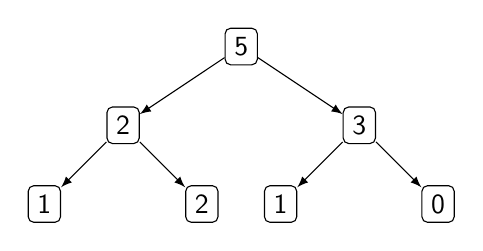
\begin{tikzpicture}[
	level 1/.style={sibling distance=30mm},
	level 2/.style={sibling distance=20mm},
	level 3/.style={sibling distance=10mm},
	level distance = 1cm,
	edge from parent/.style={->,draw},>=latex]
		\begin{scope}[every node/.style={root}]
			\node{5}
				child{node{2}
					child{node{1}}
					child{node{2}}}
				child{node{3}
					child{node{1}}
					child{node{0}}};
		\end{scope}
	\end{tikzpicture}\end{center} 
	\caption{The first four sorting operations of heapsort. The row of numbers corresponds to the
	array being sorted. The tree represents the heap.}
	\label{example-heapsort1}
\end{figure}

\begin{figure}
	\List{0, 2, 3, 1, 2, 1, 5, 7, 8, 12}
	\vspace{5mm}
	\begin{center}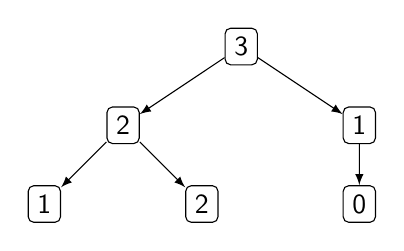
\begin{tikzpicture}[
	level 1/.style={sibling distance=30mm},
	level 2/.style={sibling distance=20mm},
	level 3/.style={sibling distance=10mm},
	level distance = 1cm,
	edge from parent/.style={->,draw},>=latex]
		\begin{scope}[every node/.style={root}]
			\node{3}
				child{node{2}
					child{node{1}}
					child{node{2}}}
				child{node{1}
					child{node{0}}};
		\end{scope}
	\end{tikzpicture}\end{center} 
	\vspace{5mm}
	\List{0, 2, 1, 1, 2, 3, 5, 7, 8, 12}
	\vspace{5mm}
	\begin{center}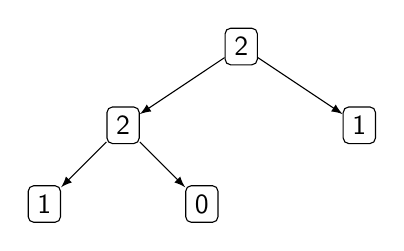
\begin{tikzpicture}[
	level 1/.style={sibling distance=30mm},
	level 2/.style={sibling distance=20mm},
	level 3/.style={sibling distance=10mm},
	level distance = 1cm,
	edge from parent/.style={->,draw},>=latex]
		\begin{scope}[every node/.style={root}]
			\node{2}
				child{node{2}
					child{node{1}}
					child{node{0}}}
				child{node{1}};
		\end{scope}
	\end{tikzpicture}\end{center} 
	\vspace{5mm}	
	\List{0, 2, 1, 1, 2, 3, 5, 7, 8, 12}
	\vspace{5mm}
	\begin{center}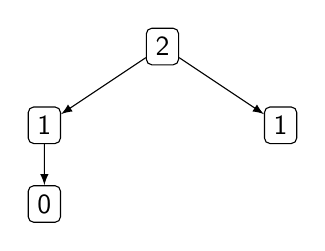
\begin{tikzpicture}[
	level 1/.style={sibling distance=30mm},
	level 2/.style={sibling distance=20mm},
	level 3/.style={sibling distance=10mm},
	level distance = 1cm,
	edge from parent/.style={->,draw},>=latex]
		\begin{scope}[every node/.style={root}]
			\node{2}
				child{node{1}
					child{node{0}}}
				child{node{1}};
		\end{scope}
	\end{tikzpicture}\end{center} 
	\vspace{5mm}
	\List{0, 1, 1, 2, 2, 3, 5, 7, 8, 12}
	\vspace{5mm}
	\begin{center}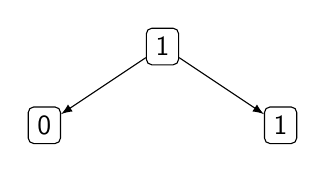
\begin{tikzpicture}[
	level 1/.style={sibling distance=30mm},
	level 2/.style={sibling distance=20mm},
	level 3/.style={sibling distance=10mm},
	level distance = 1cm,
	edge from parent/.style={->,draw},>=latex]
		\begin{scope}[every node/.style={root}]
			\node{1}
				child{node{0}}
				child{node{1}};
		\end{scope}
	\end{tikzpicture}\end{center} 
	\vspace{5mm}
	\List{1, 0, 1, 2, 2, 3, 5, 7, 8, 12}
	\vspace{5mm}
	\begin{center}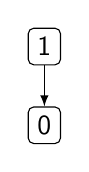
\begin{tikzpicture}[
	level 1/.style={sibling distance=30mm},
	level 2/.style={sibling distance=20mm},
	level 3/.style={sibling distance=10mm},
	level distance = 1cm,
	edge from parent/.style={->,draw},>=latex]
		\begin{scope}[every node/.style={root}]
			\node{1}
				child{node{0}};
		\end{scope}
	\end{tikzpicture}\end{center} 
	\vspace{5mm}
	\List{0, 1, 1, 2, 2, 3, 5, 7, 8, 12}
	\caption{The remaining heapsort operations. Notice how the heap gets smaller as
	the list becomes sorted from right to left.}
	\label{example-heapsort2}
\end{figure}

\pagebreak
\section{Quicksort}
Quicksort is a divide-and-conquer algorithm that divides an array over a chosen pivot and then recursively sorts the subarrays. Quicksort can be done in place and is unstable.

The Quicksort algorithm involves choosing a pivot and rearranging the elements in the array so 
that the elements less than the pivot are to its left and the elements greater than the pivot are to its 
right. This effectively splits the original array into two subarrays. There are different ways to 
implement the partition function, but normally a variation of the so-called Hoare partition is
used. 

In the Hoare partition method, a pivot is selected (the method used in this research paper merely
selects the middle element of the array, but there are many different other methods available).
The array is searched from left to right until a value is found that is larger than the pivot. The index
of this position is saved, and the array is then searched from right to left until a value is found
that is less than the pivot. At that point, the two elements are switched, ensuring their final
positions are on the correct side of the pivot. This process is completed until the left index is
greater than the right index. At this point, the array partition process has been completed.

This partitioning process is performed recursively on both subarrays until the subarrays consist
of one element, thus ensuring the array is not only partitioned, but sorted. No combination phase is 
needed, as is required with Mergesort, because the array is sorted in place. 
Figure~\ref{pseudo-quicksort} contains the pseudo code Quicksort. 
Figure~\ref{example-quicksort} demonstrates an array of numbers being sorted with Quicksort.

It is easy to see that the partitioning process itself is linear since each element of the array
is examined exactly once. However the efficiency of the entire Quicksort algorithm depends
upon the number of recursive calls that are required to complete the sort. In the best case
(which turns out to be close to the average case), the pivot's value is the median value. That is, 
after the array has been sorted, an equal number of elements will be on each side of the median. 
This divides the array in half. If the pivots for each of these subarrays is similarly selected with the
median value, the array will be divided into a total of four pieces. If this process continues,
this leads to $\log_2n$ total recursive calls. When summed with the partition operation, this is
clearly a $O(n \log n)$ operation.

However, if the value of the pivot is the smallest or the largest values of the array, 
then the size of the array will only be decreased by a one during the partition process, and the 
algorithm will end up requiring more recursive calls. In fact, if each pivot
is selected in a similar poor fashion, the partition operation will be performed on a total of $n-1$ 
subarrays, resulting in an $O(n^2)$ algorithm.

This makes the efficiency of Quicksort highly dependent upon the composition of its input
array. In fact, the recursive nature of Quicksort makes it completely unsuitable for some types
of data sets (as the measurement results described later in this paper will demonstrate). 
However, in most cases, the efficiency granted Quicksort by the Hoare partition operation makes
it an ideal sorting algorithm in most situations, and it has been incorporated into many standard
libraries.

One common situation that Quicksort does not handle very well is when an array has many 
repeating elements. Figure~\ref{example-quicksort-repeat} demonstrates the initial partitioning
of an array that has many repeating elements. As the example shows, when the pivot has a value
that repeats many times, some of the sorts are unproductive, and the resulting array is
not partitioned very well; there will be values equal to the pivot element in both subarrays.
Because Quicksort does so poorly in this type of situation, several different variations of Quicksort
were created to handle this particular situation: Dual Pivot Quicksort and Three Way Quicksort
are two such variations.

\begin{figure}
\begin{algorithmic}
	\Procedure{Quicksort}{A[left..right],left,right}
		\State $pivot \gets A[(left + right)/2]$
		\State $l \gets left$
		\State $r \gets right$
		\While{$l \le r$}
			\While{$A[l] < pivot$}
				\State $i \gets i + 1$
			\EndWhile
			\While{$A[r] > pivot$}
				\State $r \gets r - 1$
			\EndWhile
			\If{$l \le r$}
				\State $swap(A[l], A[r])$
				\State $l \gets l + 1$
				\State $r \gets r - 1$
			\EndIf
		\EndWhile
		\If{$left < r$}
			\State $quicksort(A, left, r)$
		\EndIf
		\If{$l < right$}
			\State $quicksort(A, l, right)$
		\EndIf
	\EndProcedure
\end{algorithmic}
\caption{Quicksort algorithm}
\label{pseudo-quicksort}
\end{figure}

\begin{figure}[quicksort]\begin{doublespace}
\List{s2/3, 5, 7, 1, p1/2, 12, 0, 2, 8, s3/1} 
\List{1, s2/5, 7, 1, p1/2, 12, 0, s3/2, 8, 3}
\List{1, 2, s2/7, 1, p1/2, 12, s3/0, 5, 8, 3}
\List{s2/1, p1/2, 0, s3/1, , 2, , s2/12, 7, p1/5, 8, s3/3}
\List{1, s2/2, 0, s3/1, , 2, , 3, s2/7, s3/5, 8, 12}
\List{1, 1, 0, p1/2, , 2, , 3, p1/5, 7, 8, 12}
\List{s2/1, p1/1, s3/0,, 2, , 2, , 3,, 5,, s2/7, p1/8, s3/12}
\List{0, p1/1, 1,, 2, , 2, , 3,, 5,, 7, p1/8, 12}
\List{0, 1, 1,2, 2, 3, 5, 7, 8, 12}
\caption{Quicksort: the blue and red boxes represent the values to be swapped. The 
grey box represents the pivot.}
\label{example-quicksort}
\end{doublespace}
\end{figure}

\begin{figure}\begin{doublespace}
\List{3, s2/6, 3, 6, p1/6, 8, 3, 8, 6, s3/6}
\List{3, 6, 3, s2/6, p1/6, 8, 3, 8, s3/6, 6}
\List{3, 6, 3, 6, s2/6, 8, s3/3, 8, 6, 6}
\List{3, 6, 3, 6, 3, 8, 6, 8, 6, 6}
\end{doublespace}
\caption{The first partitioning of an array with many repeating characters}
\label{example-quicksort-repeat}
\end{figure}

\section{Dual-Pivot Quicksort}
The idea behind a dual pivot is that, if partitioning into two pieces leads to an efficient
sort, then partitioning into three pieces could improve upon this efficiency. In 1975, Sedgewick
proposed a dual pivot variation of Quicksort\cite{Sedgewick75}, but it turned out to be less
efficient than Quicksort because of the additional overhead introduced by the second pivot.
Until 2009, it was assumed that any other implementations of a dual pivot Quicksort would
have similar problems. But then Vladimir Yaroslavskiy, with the help of Jon Bentley and Joshua
Bloch, came out with an implementation of Dual-Pivot Quicksort that has since been 
incorporated into Java 7 as the standard sort on primitive data types.

Dual-Pivot Quicksort tweaks the original quicksort by adding a second pivot. Two pivots are chosen, 
typically at the left and right ends of the array. If the value of the left pivot is greater than the right 
pivot, they are swapped.  

During the partitioning phase, the array is divided into four parts:
part one contains the elements less than the first pivot, part two contains the elements that are 
greater than or equal to the first pivot and less than or equal to the second pivot, part three contains 
the elements greater than the second pivot, and part four contains the elements that have not
yet been examined. As the algorithm runs, the elements in part four are sorted into their proper
location (part one, part two, or part three) until part four is empty. The first pivot is then swapped 
with the last element of part one and the second pivot is swapped with the first element of part 
three. This partitioning is then performed recursively on each of the remaining three parts of the 
array until the entire array has been sorted. 

According to Yaroslavskiy 2009\cite{Yaroslavskiy09}, Dual Pivot Quicksort requires a fewer 
average number of swaps than the classical Quicksort and thus is a more efficient algorithm.
Since then, however, there have been some other papers published that dispute this argument.
Wild 2012\cite{Wild12} contends that Dual Pivot has, in fact, fewer comparisons but 
more swaps. A recent publication, Wild 2015\cite{Wild15} compares the number of byte code
instructions of Quicksort with Yaroslavskiy's Dual Pivot algorithm and finds that the Dual Pivot
algorithm requires more byte code instructions, on average. Wild's findings, both in 2012 and 2015,
contradict Yaroslavskiy's measurements performed in 2009. The experimental findings led
to it being incorporated into Java 7 seem to indicate that it is more efficient than Quicksort. But
the reason for this efficiency seems to be somewhat in dispute, at least for the moment.
In any case, this seems to be a topic for further discussion and research.

The actual Yaroslavskiy Dual Pivot Quicksort algorithm is somewhat complicated, and
its implementation was beyond the scope of what we wanted to tackle in this paper. Therefore,
we instead implemented a simplified version of the Dual Pivot Quicksort. The pseudocode for
this algorithm is shows in Figure~\ref{pseudo-dualpivot}. Figure~\ref{example-dualpivot} contains 
an example of an array sorted using its algorithm.

\begin{figure}
\begin{algorithmic}
	\Procedure{DualPivotQS}{$A[l..r]$}
		\If{$l > r$}
  			\State \textbf{return}
		\EndIf
		\State $left \gets l$
		\State $right \gets r$
		\State $i \gets l + 1$
		\If{$A[l] > A[r]$}
			\State swap(Al], A[r])
		\EndIf
		\While{$i <= right$}
  			\If{$A[i] < A[l]$}
    				\State $swap(A[i], A[left])$
    				\State $left \gets left + 1$
				\State $i \gets i + 1$
  			\Else 
				\If{$A[r] < A[i]$}
    					\State $swap(A[i], A[right])$
    					\State $right \gets right - 1$
  				\Else
    					\State $i \gets i + 1$
				\EndIf
			\EndIf
		\EndWhile
		\State $left \gets left - 1$
		\State $swap(A[left], A[l])$
		\State $right \gets right + 1$
		\State $swap(A[right], A[r])$
		\State $DualPivotQS(l, left - 1)$
		\If{$A[left] < A[right]$}
  			\State $DualPivotQS(left + 1, right - 1)$
		\EndIf
		\State $DualPivotQS(right + 1, r)$
	\EndProcedure
\end{algorithmic}
\caption{Pseudocode for Dual Pivot Quicksort}
\label{pseudo-dualpivot}
\end{figure}

\begin{figure}\begin{doublespace}
\List{s2/3, 5, 7, 1, 2, 12, 0, 2, 8, s3/1} 
\List{1, s2/5, 7, 1, 2, 12, 0, 2, s3/8, 3}
\List{1, s2/8, 7, 1, 2, 12, 0, s3/2, 5, 3}
\List{1, 2, s2/7, 1, 2, 12, s3/0, 8, 5, 3}
\List{1, s2/2, s3/0, 1, 2, 12, 7, 8, 5, 3}
\List{s2/1, s3/0, 2, 1, 2, 12, 7, 8, 5, 3}
\List{0, 1, 2, 1, 2, s2/12, 7, 8, 5, s3/3}
\List{0, , 1, , s2/2, s3/1, 2, ,3, ,7, 8, 5, 12}
\List{0, , 1, , 1, 2, 2, ,3, ,7, s2/8, s3/5, 12}
\List{0, , 1, , 1, 2, 2, ,3, ,s2/7, s3/5, , 8, 12}
\List{0, 1, 1, 2, 2, 3, 5, 7, 8, 12}
\end{doublespace}
\caption{Dual Pivot Quicksort. The red and blue boxes represent the elements that will
be swapped next.}
\label{example-dualpivot}
\end{figure}

\section{Three Way Quicksort}
Dijkstra's Three Way Quicksort uses a single pivot, but partitions the elements into three different 
sections. During the partition process, there are four parts: elements less than the pivot, elements 
equal to the pivot, elements greater than the pivot, and the area not yet checked. An index 
advances through the area not yet checked. There are three possibilities: if the value at the 
index is less than the pivot value, the value at the index is swapped with the value at the 
left boundary and both the left boundary and the index are incremented. If the index value is 
greater than the pivot, it is swapped with the value at the right boundary, and the right boundary
is decremented. If the index value is equal to the pivot, the index is incremented. This is 
recursively done until the array has been sorted. When all elements have been partitioned,
Three Way Quicksort is called recursively on the subarray to the left of the pivot values
and the subarray to the right of the pivot values. 

In particular, this partition method handles inputs with many repeating elements. Instead of
pivot values ending up on either side of the partition where they will need to be partitioned
again, the pivot values end up in the middle of the array where they can be considered sorted.
Figure~\ref{pseudo-threeway} contains the pseudocode for Three Way Quicksort. 
Figure~\ref{example-threeway} has an example of an array being sorted with Three Way
Quicksort.

\begin{figure}
\begin{algorithmic}
	\Procedure{3WayQS}{$A[l..r]$}
		\If{ $l > r$}
			\State \textbf{return}
		\EndIf
		\State $left \gets l$
		\State $right \gets r$
		\State $i \gets l + 1$
		\State $pivotIdx \gets l$
		\State $pivotVal \gets A[pivotIdx]$
		\While{$i <= right$}
  			\If{$A[i] < pivotVal$}
				\State $swap(A[i], A[left]$
    				\State $left \gets left + 1$
    				\State $i \gets i + 1$
  			\Else
				\If{$pivotVal < A[i]$}
					\State $swap(A[i], A[right])$
    					\State $right \gets right - 1$
  				\Else
    					\State $i \gets i + 1$
				\EndIf
			\EndIf
		\EndWhile
		\State $3WayQS(l, left - 1)$
		\State $3WayQS(right + 1, r)$
	\EndProcedure
\end{algorithmic}
\caption{Pseudocode for Three Way Quicksort}
\label{pseudo-threeway}
\end{figure}

\begin{figure}[quicksort]\begin{doublespace}
	\List{p1/3, s2/5, 7, 1, 2, 12, 0, 2, 8, s3/1} 
	\List{s2/3, s3/1, 7, 1, 2, 12, 0, 2, 8, 5}
	\List{1, p1/3, s2/7, 1, 2, 12, 0, 2, s3/8, 5}
	\List{1, p1/3, s2/8, 1, 2, 12, 0, 2, s3/7, 5}
	\List{1, s2/3, s3/2, 1, 2, 12, 0, 8, 7, 5}
	\List{1, 2, s2/3, s3/1, 2, 12, 0, 8, 7, 5}
	\List{1, 2, 1, s2/3, s3/2, 12, 0, 8, 7, 5}
	\List{1, 2, 1, 2, p1/3, s2/12, s3/0, 8, 7, 5}
	\List{1, 2, 1, 2, s2/3, s3/0, 12, 8, 7, 5}
	\List{1, 2, 1, 2, 0, p1/3, 12, 8, 7, 5}
	\List{p1/1, s2/2, 1, 2, s3/0, , 3, , s2/12, s3/8, 7, 5}
	\List{s2/1, s3/0, 1, 2, 2, , 3, , 8, s2/12, s3/7, 5}
	\List{0, p1/1, 1, 2, 2, , 3, , 8, 7, s2/12, s3/5}
	\List{0, p1/1, 1, 2, 2, , 3, , 8, 7, 5, p1/12}
	\List{0, p1/1, 1, 2, 2, , 3, , s2/8, s3/7, 5, 12}
	\List{0, p1/1, 1, 2, 2, , 3, , 7, s2/8, s3/5, 12}
	\List{0, p1/1, 1, 2, 2, , 3, , 7, 5, p1/8, 12}
	\List{0, p1/1, 1, 2, 2, , 3, , s2/7, s3/5, 8, 12}
	\List{0, p1/1, 1, 2, 2, , 3, , 5, 7, 8, 12}
	\end{doublespace}
	\caption{Three Way Quicksort}\label{example-threeway}
\end{figure}

\pagebreak
\section{Introsort}
Introsort, invented by David Musser in 1997,  is another variation of Quicksort that takes a different 
approach to solving Quicksort's
shortcomings. Instead of modifying Quicksort to handle the specific inputs for which Quicksort
is particularly bad, Introsort handles the recursion problem itself. That is, there are inputs that
require a large number of recursive calls within Quicksort. During a recursive call within a 
program, the current state of the program is
saved onto the program's stack, and the function is called again. If too many recursive calls are
made, the stack will eventually fill up enough to meet the heap, which is stored at the other end
of the program's address space. When there is no space left, the program throws a stack
exception. This is sometimes called ``blowing the stack.''

When the input array into Quicksort is large, and the resulting recursive calls are deep enough,
Quicksort (and many of its variations) will blow the stack of the program. Since it may not always
be possible to know what type of input is being passed into the sort function or whether or
not that input will cause this stack problem, Introsort was created to handle the recursion problem
itself.
That is, a variable is passed to each call in order to keep track of the recursive depth. When
this depth exceeds a particular value (usually related to $\log_2$ of the original $n$, the sort 
switches over the Heapsort, a slower but more reliable algorithm.

This gives Introsort the best of both worlds; for most inputs, its speed nearly matches the
speed of Quicksort (some overhead is used to track the recursive depth variable), but when
the depth of recursion is great enough to indicate that Introsort is having trouble with the
input, the program switches over to Heapsort to complete the sort.

\begin{figure}
\begin{algorithmic}
	\Procedure{Introsort}{$A[l..r], depth$}
		\If{$length(A) \le 1$}
			\State \textbf{return}
		\EndIf
		\If{$depth = 0$}
			\State $heapsort(A)$
		\Else
			\State $p \gets partition(A,p)$
			\State $introsort(A[0..p], depth - 1)$
			\State $introsort(A[p+1..length(A) - 1], depth - 1)$
		\EndIf
	\EndProcedure
\end{algorithmic}
\end{figure}

\section{Implementation}
This project involved the implementation of six different programs in Java: Mergesort,
Heapsort, Quicksort, Dual Pivot Quicksort, Three Way Quicksort, and Introsort. Each
program was tested against XXX types of inputs including pseudo-random numbers,
sorted numbers, reverse sorted numbers, numbers with many repeats, and almost-sorted
numbers.

An abbreviated version of each program is shown in Figures~\ref{code-mergesort}-
~\ref{code-introsort}. In each case, some details have been omitted for brevity including
the declaration and initialization of variables.

Dual Pivot:
Typically dual-pivot uses insertion sort if 
the length of the array is small, but because we were testing on large arrays, we left out this 
implementation. 

The disadvantages are the same in that the worst case is ?(n2) and it is not a stable sort. An 
additional problem seems to be dealing with very large arrays that are in sorted, reverse sorted, or 
nearly sorted order. We discovered that dual-pivot quicksort suffered stack overflow at a fairly low 
array size (several thousand) and was unable to sort any of the lists that we used due to their size 
and the number of recursive calls that needed to be made.  We checked this issue with an 
implementation created by Princeton University and discovered that theirs blew up with stack 
overflow as well. Clearly, this is useful for getting rid of quadratic scenarios with regular quicksort, 
but it seems to be better used on totally random number, duplicate numbers, and smaller sorted 
arrays.

Three Way Quicksort
The advantages to the Three Way Quicksort is the same as dual sort, it is able to maintain 
?(nlogn) in situations where regular quicksort would have ?(n2). It is also sorted in place with e space 
complexity of ?(1) and maintains ?(nlogn) complexity in the average case.

The disadvantages of 3-way quicksort are that it is also not a stable sort, and it also faces some, but not
all, of the issues that Dual-Pivot sort faces with very large sorted numbers. 3-way quicksort was able to 

sort reverse numbers, but had stack overflow on sorted numbers, just like dual-pivot quicksort did. It 

was able to handle nearly sorted arrays, but ended with stack overflow when the array size increased to 
15 million. This is another algorithm that is more useful than regular quicksort in certain scenarios, but 

would be unable to keep up if very large arrays of potentially sorted data needed to be checked.
 
\begin{figure}
\begin{lstlisting}
public static Integer[] mergesort(Integer[] nums) { 
   System.arraycopy(nums,0,left,0,left.length);
   System.arraycopy(nums,left.length,right,0,right.length);
   left = mergesort(left);
   right = mergesort(right);
   nums = merge(left,right);
   return nums;
}

public static Integer[] merge(Integer[] left, Integer[] right) {
   while(lcount < left.length && rcount < right.length) {
      if(left[lcount] < right[rcount]) {
         sorted[i] = left[lcount];
         lcount++;
      }
      else {
         sorted[i] = right[rcount];
         rcount++;
      }
      i++;
   }
   System.arraycopy(left,lcount,sorted,i,left.length - lcount);
   System.arraycopy(right,rcount,sorted,i,right.length - rcount);
   return sorted;
}
\end{lstlisting}
\caption{Abbreviated version of Mergesort}
\label{code-mergesort}
\end{figure}

\begin{figure}
\begin{lstlisting}
private static void heapify(Integer[] nums,int root,int left,int right) {
   int temp = nums[left+root-1];
   while (root*2 <= right) {
      child = 2*root;
      if(child < right && nums[left+child-1] < nums[left+child]) {
        child++;
      }
      if(temp >= nums[left+child-1]) break;
      nums[left+root-1] = nums[left+child-1];
      root = child;
   }
   nums[left+root-1] = temp;
}
\end{lstlisting}
\caption{Abbreviated version of heapify phase of Heapsort}
\end{figure}

\begin{figure}
\begin{lstlisting}
public void quicksort(int left,int right){
   int pivot = nums[(left+right)/2];
   while(l<=r) {
      while(nums[l]<pivot)
         ++l;
      while(nums[r]>pivot)
         --r;
      if(l<=r) {
         swap(nums[l],nums[r])
	++l;
	--r;
      }
   }
   if(left < r)
      quicksort(left,r);
   if(l < right)
      quicksort(l,right);
}
\end{lstlisting}
\caption{Abbreviated version of Quicksort}
\end{figure}

\begin{figure}
\begin{lstlisting}
public void dual_pivot_qs(int left,int right){
   if(right <= left) return;
   int l = left+1;
   int r = right-1;
   int i = left+1;
   if(nums[left]>nums[right])
      swap(nums[left],nums[right])
   while(i <= r){
      if(nums[i] < nums[left]) {
         swap(nums[i],nums[l]
	 ++l;
	 ++i;
      }
      else if(nums[right]<nums[i]) {
         swap(nums[i],nums[r])
         --r;
      }
      else
         ++i;
   }
   --l;
   swap(nums[l],nums[left]);
   ++r;
   swap(nums[r],nums[right]);
   quicksort(left,l-1);
   if(nums[l] < nums[r])
      dual_pivot_qs(l+1,r-1);
   dual_pivot_qs(r+1,right);
}
\end{lstlisting}
\caption{Abbreviated version of Dual Pivot Quicksort}
\label{code-dualpivot}
\end{figure}

\begin{figure}
\begin{lstlisting}
public void three_way_qs(int left, int right){
  if(left >= right)
   return;
  int l = left;
  int r = right;
  int i = left + 1;		
  int pivotI = left;
  int pivotV = nums[pivotI];
  while(i <= r){
    if(nums[i] < pivotV) {
      swap(nums[i],nums[l]);
      ++l;
      ++i;
    }
    else if(pivotV < nums[i]) {
      swap(nums[i], nums[r]);
      --r;
    }
    else { 
      ++i;
    }
  }
  quicksort(left, l - 1);
  quicksort(r + 1, right);
}
\end{lstlisting}
\caption{Abbreviated version of Three Way Quicksort}
\label{code-threeway}
\end{figure}

\begin{figure}
\begin{lstlisting}
public static void introsort(Integer[] input, int maxdepth, int left, int right) {
    if(maxdepth == 0) {
      heap.heapsort(input, left, right);
    }
    int pivot = input[(left + right) / 2];
    int l = left;
    int r = right;
    while(l <= r) {
      while(input[l] < pivot)
        ++l;
      while(input[r] > pivot)
        --r;
      if(l <= r) {
        swap(input[l], input[r]);
        ++l;
        --r;
      }
    }
    if(left < r)
      introsort(input, maxdepth - 1, left, r);
    if(l < right)
      introsort(input, maxdepth - 1, l, right);
}
\end{lstlisting}
\caption{Abbreviated version of Introsort}
\label{code-introsort}
\end{figure}

\begin{figure}
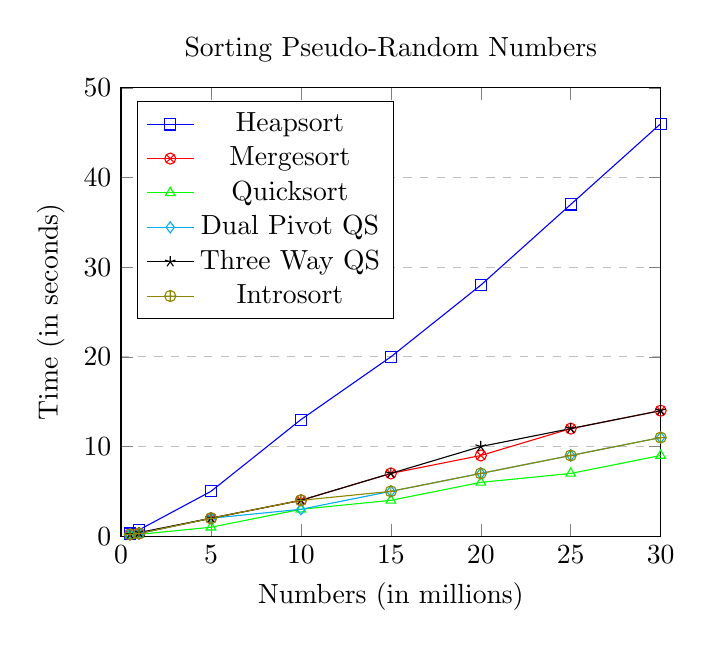
\begin{tikzpicture}
\begin{axis}[
    title={Sorting Pseudo-Random Numbers},
    xlabel={Numbers (in millions)},
    ylabel={Time (in seconds)},
    xmin=0, xmax=30,
    ymin=0, ymax=50,
    xtick={0,5,10,15,20,25,30},
    legend pos=north west,
    ymajorgrids=true,
    grid style=dashed,
]
 
\addplot[
    color=blue,
    mark=square,
    ]
    coordinates {
    (.5, .3)(1, .7)(5,5)(10,13)(15,20)(20,28)(25,37)(30,46)
    };
    \addlegendentry{Heapsort}
\addplot[
    color=red,
    mark=otimes,
    ]
    coordinates {
    (.5, .2)(1, .3)(5, 2)(10,4)(15,7)(20,9)(25,12)(30,14)
    };
    \addlegendentry{Mergesort}
\addplot[
    color=green,
    mark=triangle,
    ]
    coordinates {
    (.5,.1)(1,.2)(5,1)(10,3)(15,4)(20,6)(25,7)(30,9)
    };
    \addlegendentry{Quicksort}
\addplot[
    color=cyan,
    mark=diamond,
    ]
    coordinates {
    (.5,.2)(1,.3)(5,2)(10,3)(15,5)(20,7)(25,9)(30,11)
    };
    \addlegendentry{Dual Pivot QS}
\addplot[
    color=black,
    mark=star,
    ]
    coordinates {
    (.5,.2)(1,.4)(5,2)(10,4)(15,7)(20,10)(25,12)(30,14)
    };
    \addlegendentry{Three Way QS}
\addplot[
    color=olive,
    mark=oplus,
    ]
    coordinates {
    (.5,.2)(1,.3)(5,2)(10,4)(15,5)(20,7)(25,9)(30,11)
    };
    \addlegendentry{Introsort}
\end{axis}
\end{tikzpicture}
\end{figure}

\begin{figure}
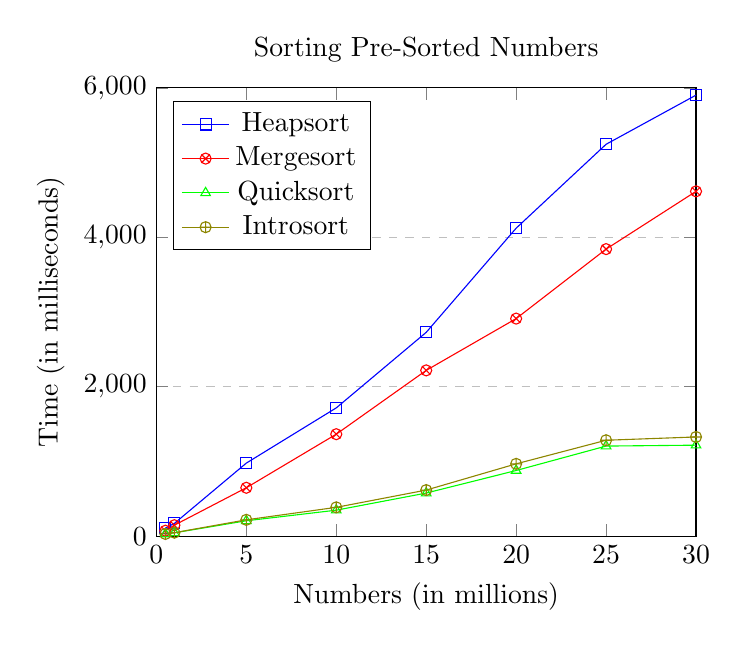
\begin{tikzpicture}
\begin{axis}[
    title={Sorting Pre-Sorted Numbers},
    xlabel={Numbers (in millions)},
    ylabel={Time (in milliseconds)},
    xmin=0, xmax=30,
    ymin=0, ymax=6000,
    xtick={0,5,10,15,20,25,30},
    legend pos=north west,
    ymajorgrids=true,
    grid style=dashed,
]
 
\addplot[
    color=blue,
    mark=square,
    ]
    coordinates {
    (.5, 107)(1, 171)(5,978)(10,1717)(15,2728)(20,4122)(25,5245)(30,5903)
    };
    \addlegendentry{Heapsort}
\addplot[
    color=red,
    mark=otimes,
    ]
    coordinates {
    (.5, 73)(1, 147)(5, 648)(10,1365)(15,2219)(20,2912)(25,3842)(30,4615)
    };
    \addlegendentry{Mergesort}
\addplot[
    color=green,
    mark=triangle,
    ]
    coordinates {
    (.5,29)(1,45)(5,206)(10,348)(15,577)(20,879)(25,1206)(30,1218)
    };
    \addlegendentry{Quicksort}
\addplot[
    color=olive,
    mark=oplus,
    ]
    coordinates {
    (.5,30)(1,47)(5,219)(10,386)(15,617)(20,968)(25,1284)(30,1328)
    };
    \addlegendentry{Introsort}
\end{axis}
\end{tikzpicture}
\end{figure}

\begin{figure}
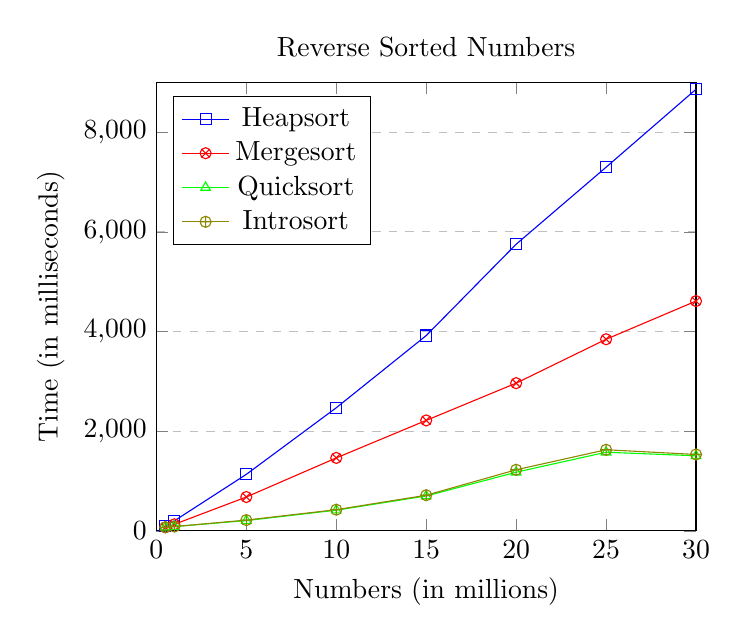
\begin{tikzpicture}
\begin{axis}[
    title={Reverse Sorted Numbers},
    xlabel={Numbers (in millions)},
    ylabel={Time (in milliseconds)},
    xmin=0, xmax=30,
    ymin=0, ymax=9000,
    xtick={0,5,10,15,20,25,30},
    legend pos=north west,
    ymajorgrids=true,
    grid style=dashed,
]
 
\addplot[
    color=blue,
    mark=square,
    ]
    coordinates {
    (.5, 99)(1, 200)(5,1133)(10,2470)(15,3919)(20,5753)(25,7299)(30,8864)
    };
    \addlegendentry{Heapsort}
\addplot[
    color=red,
    mark=otimes,
    ]
    coordinates {
    (.5,69)(1,130)(5,678)(10,1463)(15,2216)(20,2964)(25,3845)(30,4612)
    };
    \addlegendentry{Mergesort}
\addplot[
    color=green,
    mark=triangle,
    ]
    coordinates {
    (.5,72)(1,85)(5,205)(10,414)(15,699)(20,1176)(25,1577)(30,1506)
    };
    \addlegendentry{Quicksort}
\addplot[
    color=olive,
    mark=oplus,
    ]
    coordinates {
    (.5,71)(1,85)(5,215)(10,424)(15,714)(20,1225)(25,1627)(30,1532)
    };
    \addlegendentry{Introsort}
\end{axis}
\end{tikzpicture}
\end{figure}

\begin{figure}
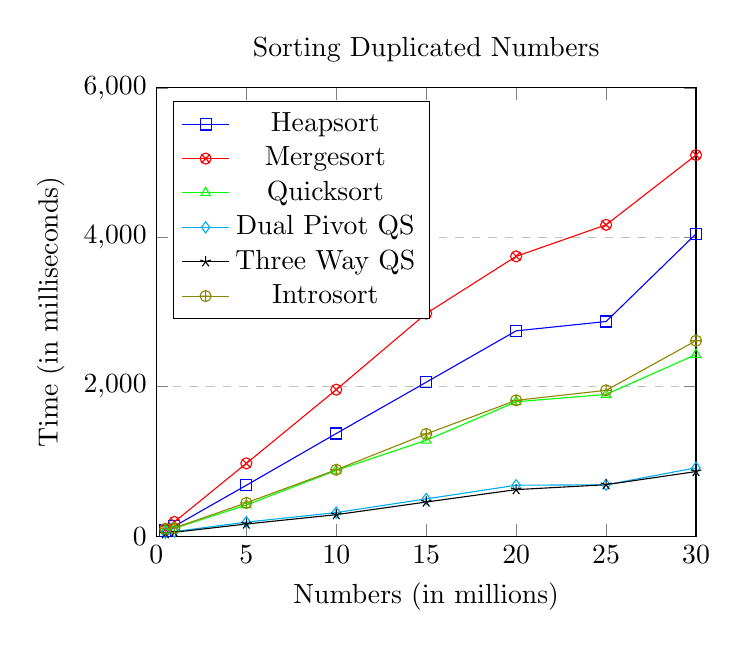
\begin{tikzpicture}
\begin{axis}[
    title={Sorting Duplicated Numbers},
    xlabel={Numbers (in millions)},
    ylabel={Time (in milliseconds)},
    xmin=0, xmax=30,
    ymin=0, ymax=6000,
    xtick={0,5,10,15,20,25,30},
    legend pos=north west,
    ymajorgrids=true,
    grid style=dashed,
]
 
\addplot[
    color=blue,
    mark=square,
    ]
    coordinates {
    (.5, 75)(1, 133)(5,681)(10,1374)(15,2060)(20,2748)(25,2873)(30,4046)
    };
    \addlegendentry{Heapsort}
\addplot[
    color=red,
    mark=otimes,
    ]
    coordinates {
    (.5, 90)(1, 191)(5, 974)(10,1961)(15,2980)(20,3745)(25,4167)(30,5101)
    };
    \addlegendentry{Mergesort}
\addplot[
    color=green,
    mark=triangle,
    ]
    coordinates {
    (.5,83)(1,105)(5,417)(10,881)(15,1283)(20,1799)(25,1897)(30,2431)
    };
    \addlegendentry{Quicksort}
\addplot[
    color=cyan,
    mark=diamond,
    ]
    coordinates {
    (.5,46)(1,62)(5,188)(10,316)(15,499)(20,682)(25,688)(30,915)
    };
    \addlegendentry{Dual Pivot QS}
\addplot[
    color=black,
    mark=star,
    ]
    coordinates {
    (.5,33)(1,52)(5,163)(10,288)(15,457)(20,623)(25,689)(30,865)
    };
    \addlegendentry{Three Way QS}
\addplot[
    color=olive,
    mark=oplus,
    ]
    coordinates {
    (.5,101)(1,111)(5,446)(10,889)(15,1368)(20,1818)(25,1952)(30,2616)
    };
    \addlegendentry{Introsort}
\end{axis}
\end{tikzpicture}
\end{figure}

\begin{thebibliography}{9}

\bibitem{Yaroslavskiy09}
  Vladimir Yaroslavskiy,
  \emph{Dual-Pivot Quicksort algorithm},
  \url{http://codeblab.com/wp-content/uploads/2009/09/DualPivotQuicksort.pdf},
  Sept 2009.
  
\bibitem{Wild12}  
Sebastian Wild and Markus E. Nebel,
Average Case Analysis of Java 7?s Dual Pivot Quicksort,
In Leah Epstein and Paolo Ferragina, editors, 
European Symposium on Algorithms 2012, 
volume 7501 of LNCS, pages 825?836. Springer, 2012,
\url{http://www.researchgate.net/profile/Sebastian_Wild/publication/230766496_Average_Case_Analysis_of_Java_7%27s_Dual_Pivot_Quicksort/links/09e415040f44330424000000.pdf}

\bibitem{Wild15}
Sebastian Wild, Markus E. Nebel, and Ralph Neininger,
Average Case and Distributional Analysis of Dual-Pivot Quicksort,
arXiv:1304.0988v3, Feb 2015

\bibitem{Sedgewick75}
Sedgewick, R.: Quicksort. PhD Thesis, Stanford University (1975)
\end{thebibliography}
\end{document}
